% https://tex.stackexchange.com/a/61814/23046
\tikzset {
  myarrow/.style= {-{Stealth[scale=1.0]}},
  mycircle/.style= {circle,draw=black,minimum size=0.7cm},
}

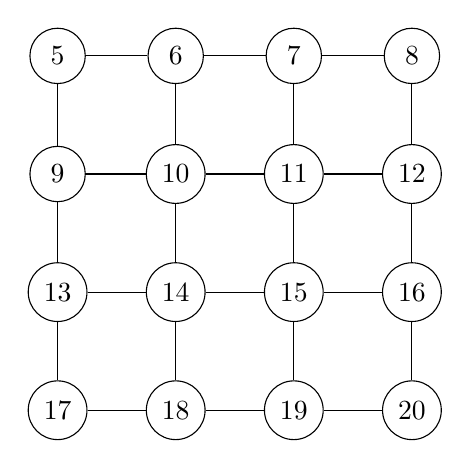
\begin{tikzpicture}[darkstyle/.style={circle,draw,minimum size=20}]
  \foreach \x in {0,...,3}
    \foreach \y in {0,...,3} 
        {\pgfmathtruncatemacro{\label}{\x - 4 *  \y +17}
        \node [darkstyle]  (\x\y) at (1.5*\x,1.5*\y) {\label};} 
  \foreach \x in {0,...,3}
    \foreach \y [count=\yi] in {0,...,2}  
      \draw (\x\y)--(\x\yi) (\y\x)--(\yi\x) ;
\end{tikzpicture}

